\begin{figure*}[t]
\centering
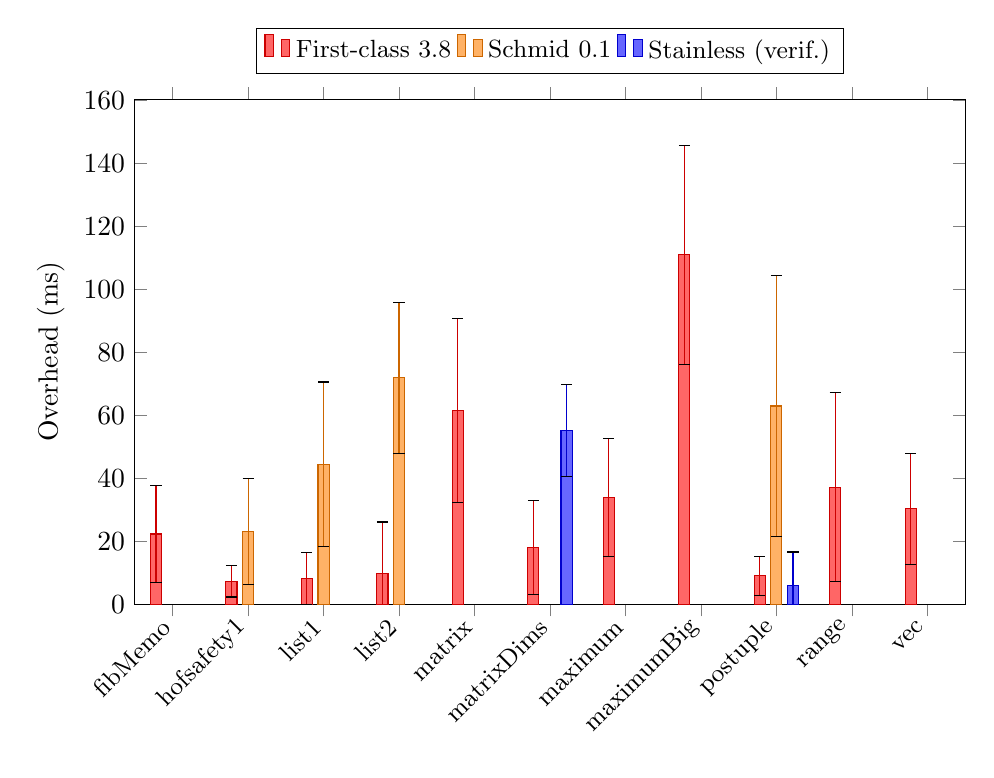
\begin{tikzpicture}
\begin{axis}[
    ybar,
    bar width=4pt,
    width=\textwidth,
    height=8cm,
    ylabel={Overhead (ms)},
    symbolic x coords={fibMemo, hofsafety1, list1, list2, matrix, matrixDims, maximum, maximumBig, postuple, range, vec},
    xtick=data,
    x tick label style={rotate=45, anchor=east, font=\small},
    legend style={at={(0.5,1.05)}, anchor=south, legend columns=3, font=\small},
    ymin=0,
    enlarge x limits=0.05,
    every node near coord/.style={font=\tiny},
]
\addplot[fill=red!60, draw=red!80!black, error bars/.cd, y dir=both, y explicit]
  coordinates {
    (fibMemo, 22.4) +- (0, 15.3)
    (hofsafety1, 7.4) +- (0, 5.0)
    (list1, 8.3) +- (0, 8.2)
    (list2, 10.0) +- (0, 16.2)
    (matrix, 61.6) +- (0, 29.1)
    (matrixDims, 18.1) +- (0, 14.8)
    (maximum, 34.0) +- (0, 18.6)
    (maximumBig, 110.9) +- (0, 34.8)
    (postuple, 9.2) +- (0, 6.2)
    (range, 37.2) +- (0, 30.0)
    (vec, 30.4) +- (0, 17.6)
  };
\addlegendentry{First-class 3.8}
\addplot[fill=orange!60, draw=orange!80!black, error bars/.cd, y dir=both, y explicit]
  coordinates {
    (hofsafety1, 23.3) +- (0, 16.8)
    (list1, 44.5) +- (0, 26.1)
    (list2, 71.9) +- (0, 24.0)
    (postuple, 63.0) +- (0, 41.3)
  };
\addlegendentry{Schmid 0.1}
\addplot[fill=blue!60, draw=blue!80!black, error bars/.cd, y dir=both, y explicit]
  coordinates {
    (matrixDims, 55.1) +- (0, 14.6)
    (postuple, 6.0) +- (0, 10.7)
  };
\addlegendentry{Stainless (verif.)}
\end{axis}
\end{tikzpicture}
\caption{Compilation time overhead in milliseconds compared to the respective baseline (Base~3.8 or Base~0.1). Error bars show the 95\% confidence interval.}
\label{fig:bench-overhead}
\end{figure*}